\documentclass{report}

\usepackage{graphicx}
\usepackage{caption}
\usepackage{subcaption}
\usepackage{amsmath}
\usepackage{amsfonts}
\captionsetup{justification=centerlast, margin=0.5cm}
\usepackage{verbatim}
\usepackage{etoolbox}
\usepackage{mathptmx}
\patchcmd{\abstract}{\scshape\abstractname}{\textbf{\abstractname}}{}{}

\usepackage[latin1]{inputenc}
\usepackage{tikz}
\usetikzlibrary{shapes,arrows}

\begin{document}


Abstract--We present an Android application for scanning LaTeX documents to determine the logical layout of the document. The algorithm first prepares the image for processing, then determines where text and figures are within a document, and finally classifies these various components of a document. 


\section{Introduction}
One popular method of producing aesthetically pleasing PDF documents including diverse contents is LaTeX. LaTeX is a low-level markup and programming language that allows high flexibility for designing placement of text and figures, as well as overall document structure. However, this precision is hard to reproduce; once a PDF document is generated, there is no way in general to access the code used to generate the document. In particular, it is very difficult to recreate the template used to design a document. This project aims to analyze the layout of a PDF document in order to simplify the generation of LaTeX templates. 

Images are taken on an Android device and sent to a server to be processed (Terry what are the details on the server stuff?) Once sent to the server, it is processed in a combination of Matlab and Java, and the final output is saved on the server.  The algorithm is comprised of 3 main steps: preprocessing, detecting maximal white rectangles, and classifying components of the document. 

\tikzstyle{block} = [rectangle, draw, fill=blue!20,text width=6em, text centered, rounded corners, minimum height=4em]
\tikzstyle{line} = [draw, -latex']


\begin{tikzpicture}[node distance = 3cm, auto]
% Place nodes
\node [block] (droid) {Android image capture};
\node [block, right of=droid] (binarize) {Binarization};
\node [block, right of=binarize] (skew) {Skew Correction};
\node [block, right of=skew] (margin) {Margin Removal};
\node [block,below of=margin] (mwrCC) {Preprocess Connected Components};
\node [block, left of=mwrCC] (mwrTree) {Maximal White Rectangles};
\node [block, left of=mwrTree] (mwrPost) {Postprocess White Rectangles};
\node [block, left of=mwrPost] (proj) {Analyze Horizontal Projections};
\node [block, below of=proj] (feat) {Global and Local Feature Comparison};
% Draw edges
\draw[->] (droid) -- (binarize);
\draw[->] (binarize) -- (skew);
\draw[->] (skew) -- (margin) ;
\draw[->] (margin) -- (mwrCC);
\draw[->] (mwrCC) -- (mwrTree);
\draw[->] (mwrTree) -- (mwrPost);
\draw[->] (mwrPost) -- (proj);
\draw[->] (proj) -- (feat);

\end{tikzpicture}

\section{Preprocessing}
Before analyzing the image, a reliable binarized representation of the image must be found to allow for proper interpretation of various components of a document. To optimally apply further document analysis, the image must be vertically aligned without a background. The image is captured with a mobile phone, and the document in the picture may be rotated or have low contrast. This section discusses our method of addressing these concerns in order to prepare the image for layout analysis.

\subsection{Binarization}
Lighting conditions may be uneven, so adaptive Otsu thresholding is used to binarize segments of the image. Overlapping windows of a fixed size are applied to the image, and for each window, the variance is compared to some threshold to determine whether to apply the Otsu threshold. This threshold is partially determined by the mean and variance of the entire image, since images that are taken with low lighting levels will have lower means and variances. After computing for each window, any pixels that have been evaluated as black more than twenty percent of the time are determined to be black.

\subsection{Skew Detection}
Images taken at an angle must be rotated so that text lines are parallel to the image edges. The Hough transform is used to determine the angle to which the image is rotated. Rather than applying the Hough transform to the whole image (which will detect lines that stretch diagonally across text, as well as dominant lines in the background), we apply the Hough transform to smaller portions of the image. We determine which regions are most likely to be text by evaluating the variance, and we take the Hough transform of regions where the variance is high.  \\
For each window, we find the histogram of angles, and sum the contributions. We assume that the image will be rotated by an angle less than forty-five degrees. Because of this, we can combine the contributions of perpendicular lines; a page with text going in one direction will often have lines perpendicular to the text, whether those lines represent the edges of the paper or the edges of figures. When the input angle is constrained, we can interpret perpendicular lines as representing the same input angle. We rotate the image by the angle that occurs most often in this new histogram of combined perpendicular lines.


\begin{figure}[H]%
\setcounter{subfigure}{0}
\centering
\begin{subfigure}{.5\columnwidth}
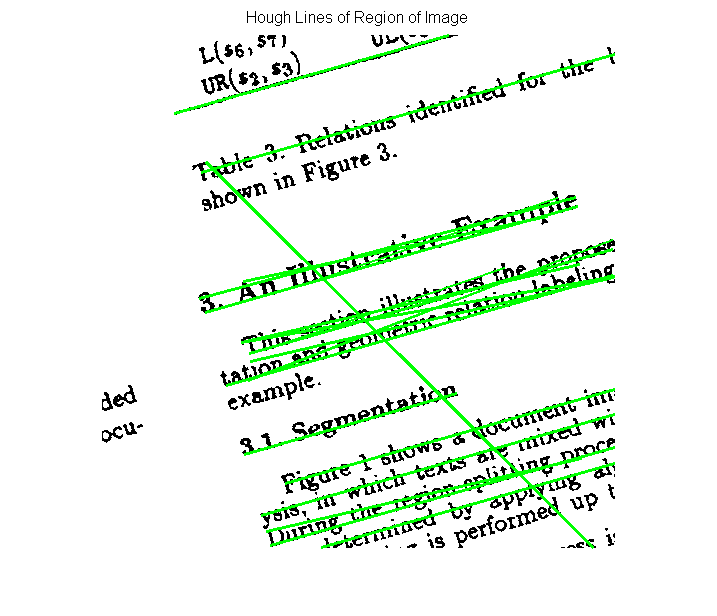
\includegraphics [width=\columnwidth]{HoughLinesEx.png}
\subcaption{Detecting Hough Transform lines of small portions of an image.}
\end{subfigure}
\hfill%
\begin{subfigure}{.5\columnwidth}
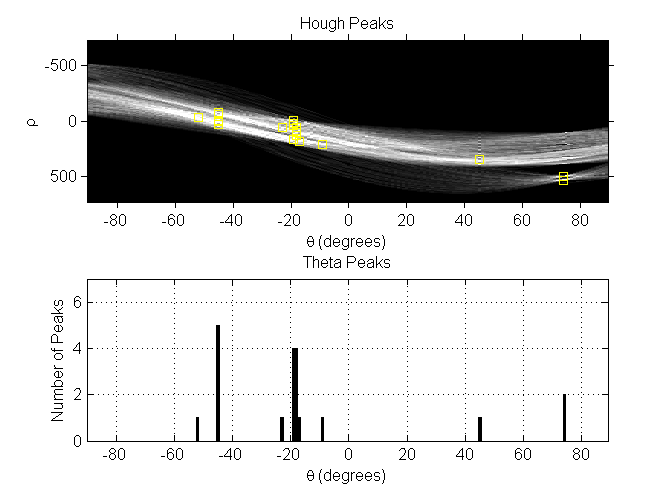
\includegraphics [width=\columnwidth]{HoughPeaksEx.png}
\subcaption{Theta Values of Hough Peaks}
\end{subfigure}

\end{figure}


\subsection{Background and Margin Removal}
To remove the background, we find the edges of the document. If the background is in contrast with the paper, binarization will detect high variance at the edges of the document, and create dark edges around the document. We find these dark edges by creating a histogram detailing the longest consecutive line of dark pixels for each row and column, and find where the number consecutive dark pixels is greater than average, which occurs at the longer stripes across the edges. Once we have determined the boundaries of the paper, we must then remove the margin. We then apply a median filter to denoise the image, and find the first and last rows and columns with black pixels to remove the margin.



\end{document}
